\documentclass[14pt]{beamer}
\usepackage[utf8]{inputenc}
\usepackage{tikz}
\usepackage{amsmath}
\usepackage{graphicx}
\usepackage{subcaption}
\usepackage{multirow}
\usepackage{multicol}
\usepackage{float,graphicx}
\usetikzlibrary{shadings, patterns, shapes.geometric}

\tikzstyle{myBox} = [rectangle, text centered, text width=4cm, draw]
\tikzstyle{node} = [circle,draw,text centered,radius=.05cm]
\tikzstyle{parallelo} = [trapezium, trapezium left angle=70, trapezium right angle=110,text width=7cm,draw]
\tikzstyle{decision} = [diamond,aspect=3,draw]

\usepackage{color}
\usepackage[skins]{tcolorbox}
\usepackage{array}


% color theme
\definecolor{bgcolor}{rgb}{0.015, 0.15, 0.23}
\definecolor{primary}{rgb}{0.88, 0.86, 0.75}
\definecolor{accent}{rgb}{0.42, 0.62, 0.6}
\definecolor{darkaccent}{rgb}{0.3, 0.48, 0.5}
\definecolor{darkeraccent}{rgb}{0.15, 0.4, 0.42}



% palette colors
\setbeamercolor{palette primary}{bg = accent, fg = bgcolor}
\setbeamercolor{palette secondary}{bg = darkaccent, fg = white}
\setbeamercolor{palette tertiary}{bg = darkeraccent, fg = primary}
\setbeamercolor{palette quaternary}{bg = darkaccent, fg = white}

\setbeamercolor{background canvas}{bg = bgcolor}
\setbeamercolor{title}{bg = darkaccent, fg = white}
\setbeamercolor{author}{fg = white}
\setbeamercolor{date}{fg = white}
\setbeamercolor{frametitle}{bg = primary, fg = bgcolor}

\setbeamercolor{section in toc}{fg = white}
\setbeamercolor{section number projected}{bg = accent, fg = bgcolor}
\setbeamercolor{subsection in toc}{fg = white}
\setbeamercolor{subsection number projected}{bg = accent, fg = bgcolor}
\setbeamercolor{item}{fg = darkaccent}
\setbeamercolor{subitem}{fg = accent}
\setbeamercolor{description item}{fg = white}
\setbeamercolor{caption}{fg = white}
\setbeamercolor{caption name}{fg = accent}

% font theme
\usefonttheme{default}
\setbeamerfont{title}{size = \LARGE}
\setbeamerfont{frametitle}{size = \Large}
\setbeamerfont{section/subsection in toc}{size = \Large}
\setbeamerfont{section number projected}{series = \bfseries}
\setbeamerfont{normal text}{size = \Large}

% inner theme
\useinnertheme[shadow]{rounded}
\useoutertheme{infolines}
\setbeamertemplate{itemize items}[square]
\setbeamertemplate{enumerate items}[circle]
\setbeamertemplate{section in toc}[circle]
\setbeamertemplate{subsection in toc}[square]
\setbeamertemplate{subsubsection in toc}[square]

% Standard block
\setbeamercolor{block title}{fg = white, bg = darkaccent}
\setbeamercolor{block body}{bg = primary, fg = bgcolor}
\setbeamercolor{normal text}{fg = white}




\tcbset{width=\textwidth, height=0.5\textheight, halign=center, valign=center, boxrule=0pt, colback=darkaccent, coltext=white}

\title[A* search]{A presentaion on A* search algorithm}
\author[1605094 \and 1605102 \and 1605110]{Priyeta Saha - 1605094 \and \\Tasnim Rahman - 1605102 \and \\Syed Muhammad - 1605110}
\date{\today}


\makeatletter
\newenvironment{withoutheadline}{
	\setbeamertemplate{headline}[default]
	\def\beamer@entrycode{\vspace*{-\headheight}}
}{}
\makeatother


\begin{document}
\begin{withoutheadline}
	\frame{\titlepage}
\end{withoutheadline}

\begin{withoutheadline}
	\begin{frame}
		\frametitle{Table Of Contents}
		\begin{multicols}{2}
			\tableofcontents
		\end{multicols}
	\end{frame}
\end{withoutheadline}

\section{Introduction}
\begin{frame}{Introduction}
	\begin{figure}[h]
	\centering
		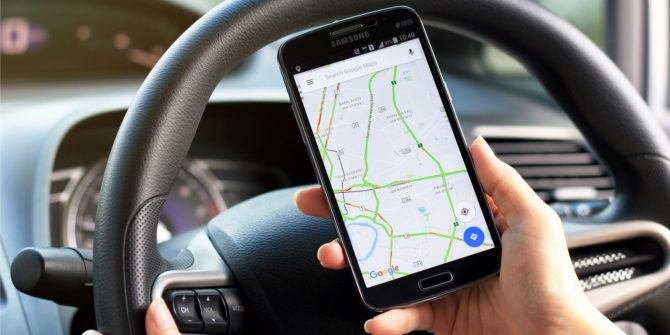
\includegraphics[width=0.8\textwidth, height=0.6\textheight]{GPS.jpeg}
		\caption{Using Navigation Assistants}
		\label{pic:GPS}
	\end{figure}
\end{frame}

\section{Definition}
\begin{frame}{Definition}
	\begin{block}{\centering What is Graph Traversal?}
		Graph traversal (also known as graph search) refers to the process of visiting (checking and/or updating) each vertex in a graph. 
	\end{block}
\end{frame}
\begin{frame}{Definition}
	\begin{figure}[h]
	\centering
		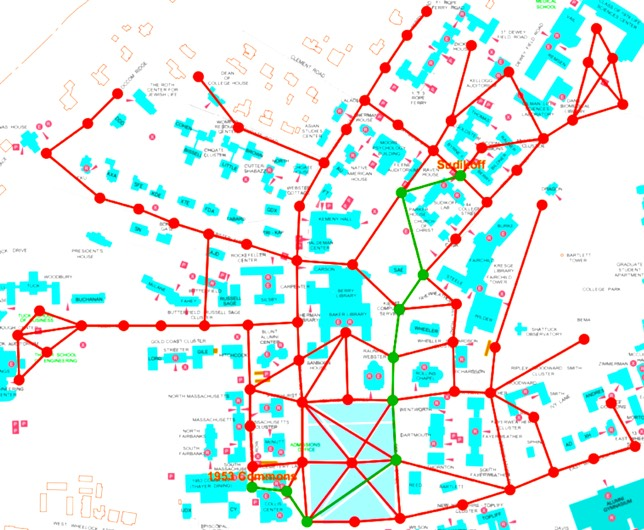
\includegraphics[width=0.6\textwidth, height=0.6\textheight]{mapgraph.jpg}
		\caption{Using Graph Traversal Algorithms}
		\label{pic:GraphTraversal}
	\end{figure}
\end{frame}


\begin{frame}{Definition}
	\begin{block}{\centering What is A* search?}
		A* search is a path-finding and graph traversal algorithm which is basically an evolution of Dijkstra's algorithm
	\end{block}
\end{frame}

\section{Why A* search?}
\begin{frame}{Why A* search?}
	As we have already mentioned, A* search is basically a modification of Dijkstra's algorithm. 
	\begin{itemize}
		\item<1-> But why do we need A* search? 
		\item<2-> What are the benefits of A* over Dijkstra's algorithm or other such algorithms which validates the modification?
	\end{itemize}
\end{frame}
	
\section{A* search Overview}
\begin{frame}{A* search Overview}
	To answer that question we first need to know how the A* search algorithm works
	\begin{itemize}
		\item<1-> You see, Dijkstra's algorithm is a greedy algorithm and so it always immediately chooses the best possible path at every step 
		\item<2-> Even if the chosen path strays away from the destination, it isn't smart enough to detect that 
		\item<3-> That's why it needs to visit a lot more nodes to come to a conclusive decision
	\end{itemize}
\end{frame}
\begin{frame}
	\begin{figure}[h]
	\centering
		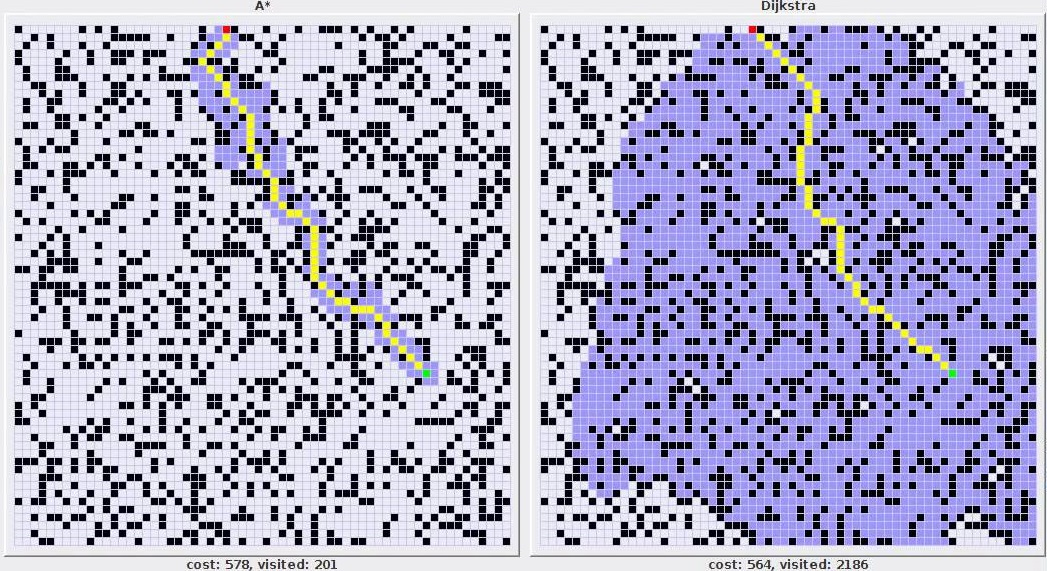
\includegraphics[scale=0.4]{avsdijkstra.jpg}
		\caption{A* search vs Dijkstra}
		\label{pic:avsdijkstra}
	\end{figure}
\end{frame}

\begin{frame}
	\begin{block}{\centering How does A* manage to be this efficient?}
		\centering
		\large \textbf {HEURISTICS}
	\end{block}
\end{frame}

\section{Heuristics}
\begin{frame}{What is Heuristics?}
	
	\begin{itemize}
		\item<1-> Heuristics is an approach to problem solving, learning, or discovery
		\item<2-> It employs a practical method not guaranteed to be optimal or perfect
		\item<3-> But it is sufficient for the immediate goals
		\begin{figure}[H]
		    \centering
		    
\includegraphics[width = .5\textwidth, height=0.35\textheight]{brain.jpg}
		    \caption{Using Heuristics}
	\end{figure}

	\end{itemize}

\end{frame}

\begin{frame}{Let's come back to this diagram again}
	\begin{figure}[h]
	\centering
		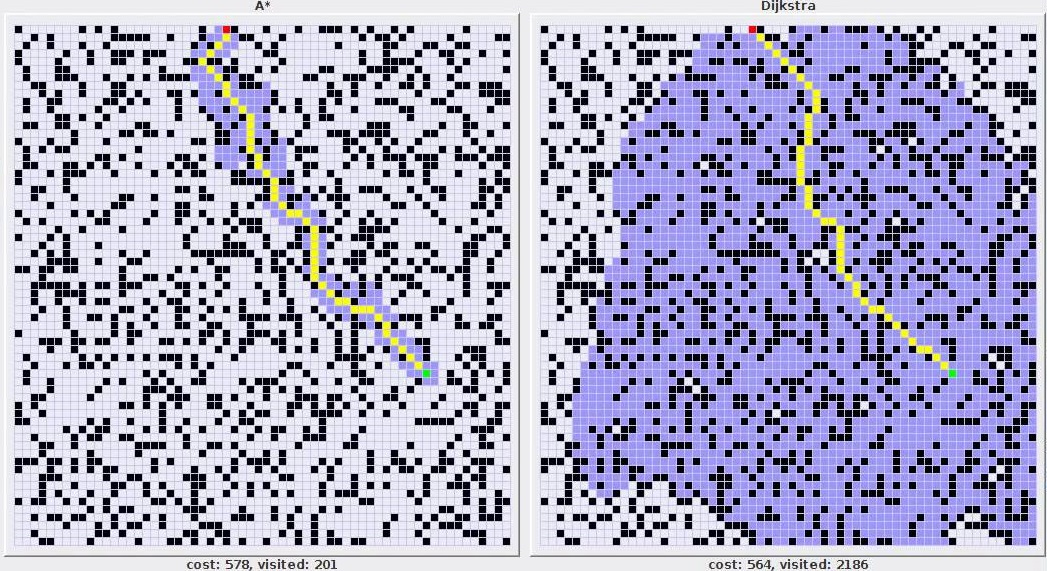
\includegraphics[scale=0.4]{avsdijkstra.jpg}
		\caption{A* search vs Dijkstra}
	\end{figure}
\end{frame}

\begin{frame}
	
	\begin{itemize}
		\item<1-> How is Heuristics used in A* search? 
		\item<2-> It can be of many different kinds
		\item<3-> For example, the Euclidean distance can be an obvious one
		\item<4-> The shorter the Euclidean distance of a node from the destination the more likely it is to be included in the optimal path
	\end{itemize}

\end{frame}

\begin{frame}
	\begin{figure}[h]
	\centering
		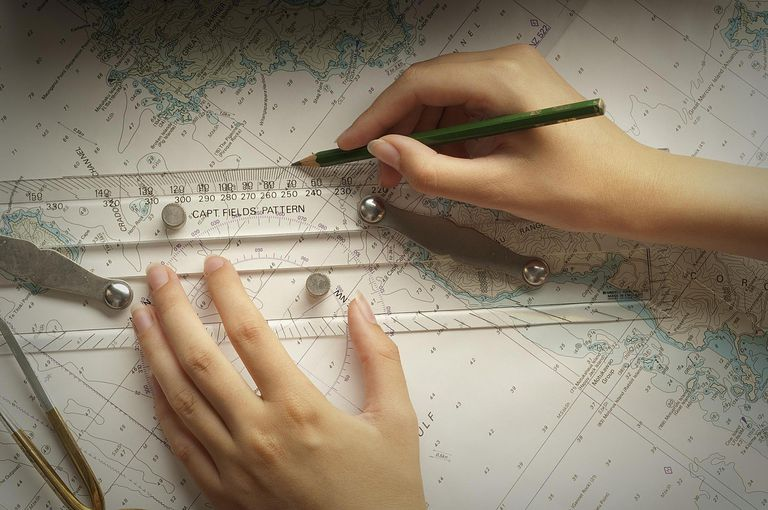
\includegraphics[scale=0.4]{mapping.jpeg}
		\caption{Using Euclidean Distance as a Heuristic measure}
		\label{pic:mapping}
	\end{figure}
\end{frame}













\section{A* Search Algorithm}
\begin{frame}{A* Search Algorithm}
	\begin{figure}[h]
	\centering
	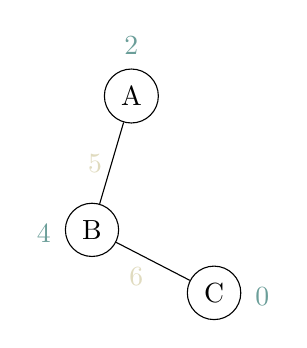
\begin{tikzpicture}

	\node[node](a) {A};
	\node[node,below of=a,yshift=-0.7cm,xshift=-0.5cm](b) {B};
	\node[node,below of=b,right of=a,yshift=-1.5cm,xshift=0.05cm](c){C};

	
	\draw[-] node[above,yshift=.4cm]{\color{accent}{2}}(a) -- node[left]{\color{primary}{5}}(b)node[left,xshift=-.4cm,yshift=-.05cm]{\color{accent}{4}};
	\draw[-] (b)--node[left,yshift=-0.2cm]{\color{primary}{6}}(c)node[right,xshift=.4cm,yshift=-.05cm]{\color{accent}{0}};

	\end{tikzpicture}
	
\end{figure}
\center f(n) = \color{primary}{d(n)} + \color{accent}{h(n)}

\end{frame}


\begin{frame}{Flow Chart}

\begin{figure}[h]
	\centering
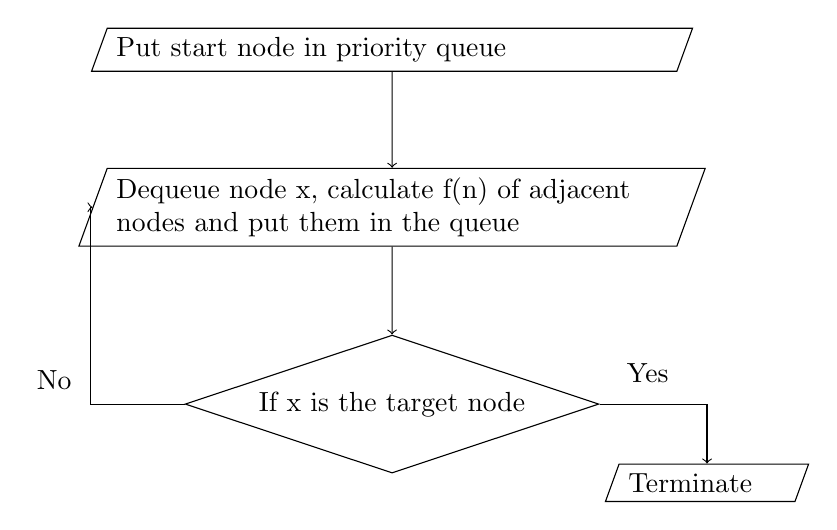
\begin{tikzpicture}
\node [parallelo](p1){Put start node in priority queue};
\node [parallelo,below of=p1,yshift=-1cm](p2){Dequeue node x, calculate f(n) of adjacent nodes and put them in the queue};
\node [decision,below of=p2,yshift=-1.5cm](d1){If x is the target node};
\node [parallelo,text width=2cm,below of=d1,xshift=4cm](p3){Terminate};


\draw[->](d1.west)node[right,xshift=-2cm,yshift=.3cm]{No}-- ++(-1.2,0)|-(p2.west);
\draw[->](d1.east)node[left,xshift=1cm,yshift=.4cm]{Yes} -- ++(.4,0)-|(p3);
\draw[->](p1)--(p2);
\draw[->](p2)--(d1);

\end{tikzpicture}
\end{figure}

\end{frame}

\begin{frame}{Example}

		Graph
		\begin{figure}[h]
			\centering
			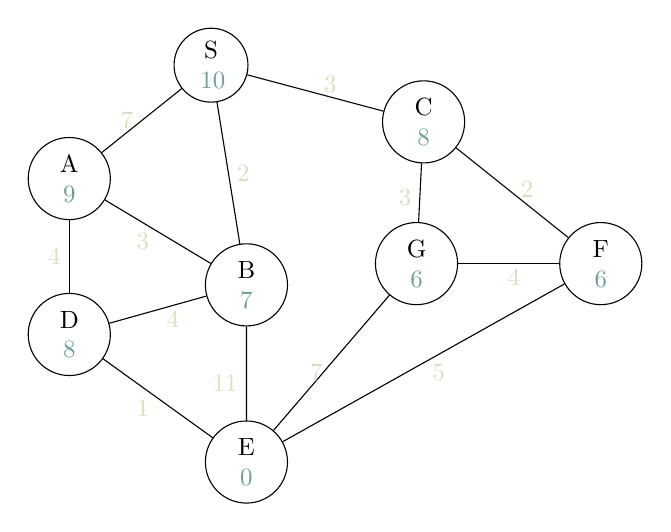
\begin{tikzpicture}[scale=0.9, every node/.style={transform shape}]
			\node [node,text width=0.3cm](s){S \color{accent}{10}};	
			\node [node,xshift=-2cm,yshift=-.6cm,below of=s,text width=0.5cm](a){A \color{accent}{9}};
			\node [node,below of=a,xshift=2.5cm,yshift=-.5cm,text width=0.5cm](b){B \color{accent}{7}};
			\node [node,below of=a,yshift=-1.2cm,text width=0.5cm](d){D \color{accent}{8}};
			\node [node,below of=s,xshift=3cm,yshift=.2cm,text width=0.5cm](c){C \color{accent}{8}};
			\node [node,below of=c,xshift=2.5cm,yshift=-1cm,text width=0.5cm](f){F \color{accent}{6}};
			\node [node,below of=c,xshift=-0.1cm,yshift=-1cm,text width=0.5cm](g){G \color{accent}{6}};
			\node [node,below of=b,yshift=-1.5cm,text width=0.5cm](e){E \color{accent}{0}};
			
			\draw[-](s)--node[left]{\color{primary}{7}}(a);
			\draw[-](s)--node[right]{\color{primary}{2}}(b);
			\draw[-](s)--node[right,yshift=.12cm]{\color{primary}{3}}(c);
			\draw[-](a)--node[left,yshift=-.14cm]{\color{primary}{3}}(b);
			\draw[-](a)--node[left]{\color{primary}{4}}(d);
			\draw[-](b)--node[right,yshift=-.14cm]{\color{primary}{4}}(d);
			\draw[-](b)--node[left,yshift=-.14cm]{\color{primary}{11}}(e);
			\draw[-](d)--node[left,yshift=-.14cm]{\color{primary}{1}}(e);
			\draw[-](c)--node[right,yshift=.05cm]{\color{primary}{2}}(f);
			\draw[-](c)--node[left,yshift=-.06cm]{\color{primary}{3}}(g);
			\draw[-](f)--node[right,xshift=-.14cm,yshift=-.2cm]{\color{primary}{4}}(g);
			\draw[-](f)--node[right,yshift=-.14cm]{\color{primary}{5}}(e);
			\draw[-](g)--node[left,yshift=-.14cm]{\color{primary}{7}}(e);
			\end{tikzpicture}
			
		\end{figure}

\end{frame}



\begin{frame}{Example}

\begin{columns}
\column{0.6\textwidth}

\begin{figure}[h]
	
	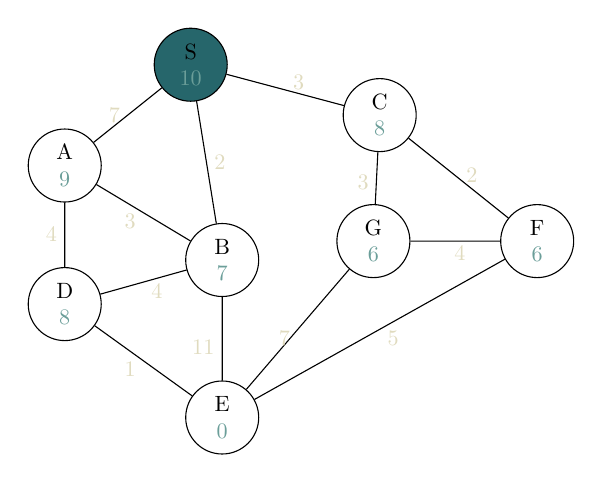
\begin{tikzpicture}[scale=0.8, every node/.style={transform shape}]
	\node [node,text width=0.5cm,fill=darkeraccent](s){S \color{accent}{10}};	
	\node [node,xshift=-2cm,yshift=-.6cm,below of=s,text width=0.5cm](a){A \color{accent}{9}};
	\node [node,below of=a,xshift=2.5cm,yshift=-.5cm,text width=0.5cm](b){B \color{accent}{7}};
	\node [node,below of=a,yshift=-1.2cm,text width=0.5cm](d){D \color{accent}{8}};
	\node [node,below of=s,xshift=3cm,yshift=.2cm,text width=0.5cm](c){C \color{accent}{8}};
	\node [node,below of=c,xshift=2.5cm,yshift=-1cm,text width=0.5cm](f){F \color{accent}{6}};
	\node [node,below of=c,xshift=-0.1cm,yshift=-1cm,text width=0.5cm](g){G \color{accent}{6}};
	\node [node,below of=b,yshift=-1.5cm,text width=0.5cm](e){E \color{accent}{0}};
	
	\draw[-](s)--node[left]{\color{primary}{7}}(a);
	\draw[-](s)--node[right]{\color{primary}{2}}(b);
	\draw[-](s)--node[right,yshift=.12cm]{\color{primary}{3}}(c);
	\draw[-](a)--node[left,yshift=-.14cm]{\color{primary}{3}}(b);
	\draw[-](a)--node[left]{\color{primary}{4}}(d);
	\draw[-](b)--node[right,yshift=-.14cm]{\color{primary}{4}}(d);
	\draw[-](b)--node[left,yshift=-.14cm]{\color{primary}{11}}(e);
	\draw[-](d)--node[left,yshift=-.14cm]{\color{primary}{1}}(e);
	\draw[-](c)--node[right,yshift=.05cm]{\color{primary}{2}}(f);
	\draw[-](c)--node[left,yshift=-.06cm]{\color{primary}{3}}(g);
	\draw[-](f)--node[right,xshift=-.14cm,yshift=-.2cm]{\color{primary}{4}}(g);
	\draw[-](f)--node[right,yshift=-.14cm]{\color{primary}{5}}(e);
	\draw[-](g)--node[left,yshift=-.14cm]{\color{primary}{7}}(e);
	\end{tikzpicture}
	
\end{figure}
\column{0.4\textwidth}
\begin{figure}[h]
Priority Queue\\*
	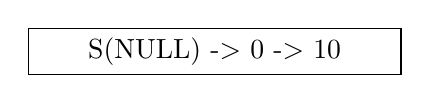
\begin{tikzpicture}
	\node [myBox, text width=4.5cm](b1){\text{S(NULL) -$>$	0 -$>$ 10}};
	\end{tikzpicture}
	
\end{figure}

\end{columns}
\end{frame}


\begin{frame}{Example}

\begin{columns}
	\column{0.6\textwidth}
	
	\begin{figure}[h]
		
		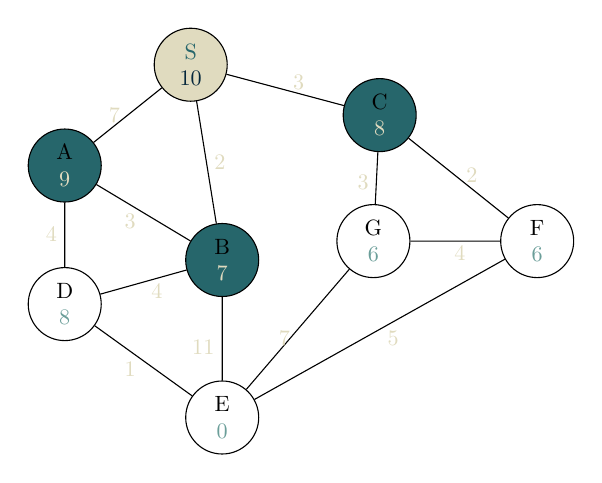
\begin{tikzpicture}[scale=0.8, every node/.style={transform shape}]
		\node [node,text width=0.5cm,fill=primary, text=darkeraccent](s){S \color{bgcolor}{10}};	
		\node [node,xshift=-2cm,yshift=-.6cm,below of=s,text width=0.5cm,fill=darkeraccent](a){A \color{primary}{9}};
		\node [node,below of=a,xshift=2.5cm,yshift=-.5cm,text width=0.5cm,fill=darkeraccent](b){B \color{primary}{7}};
		\node [node,below of=a,yshift=-1.2cm,text width=0.5cm](d){D \color{accent}{8}};
		\node [node,below of=s,xshift=3cm,yshift=.2cm,text width=0.5cm,fill=darkeraccent](c){C \color{primary}{8}};
		\node [node,below of=c,xshift=2.5cm,yshift=-1cm,text width=0.5cm](f){F \color{accent}{6}};
		\node [node,below of=c,xshift=-0.1cm,yshift=-1cm,text width=0.5cm](g){G \color{accent}{6}};
		\node [node,below of=b,yshift=-1.5cm,text width=0.5cm](e){E \color{accent}{0}};
		
		\draw[-](s)--node[left]{\color{primary}{7}}(a);
		\draw[-](s)--node[right]{\color{primary}{2}}(b);
		\draw[-](s)--node[right,yshift=.12cm]{\color{primary}{3}}(c);
		\draw[-](a)--node[left,yshift=-.14cm]{\color{primary}{3}}(b);
		\draw[-](a)--node[left]{\color{primary}{4}}(d);
		\draw[-](b)--node[right,yshift=-.14cm]{\color{primary}{4}}(d);
		\draw[-](b)--node[left,yshift=-.14cm]{\color{primary}{11}}(e);
		\draw[-](d)--node[left,yshift=-.14cm]{\color{primary}{1}}(e);
		\draw[-](c)--node[right,yshift=.05cm]{\color{primary}{2}}(f);
		\draw[-](c)--node[left,yshift=-.06cm]{\color{primary}{3}}(g);
		\draw[-](f)--node[right,xshift=-.14cm,yshift=-.2cm]{\color{primary}{4}}(g);
		\draw[-](f)--node[right,yshift=-.14cm]{\color{primary}{5}}(e);
		\draw[-](g)--node[left,yshift=-.14cm]{\color{primary}{7}}(e);
		\end{tikzpicture}
		
	\end{figure}
	\column{0.4\textwidth}
	\begin{figure}[h]
		Priority Queue\\*
		  
		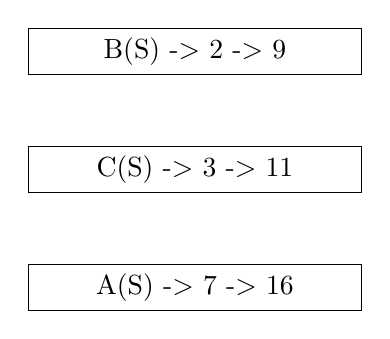
\begin{tikzpicture}
		\node [myBox](b1){\text{B(S) -$>$	2 -$>$ 9}};
		\node [myBox,below of=b1,yshift=-.5cm](b2){\text{C(S) -$>$	3 -$>$ 11}};
		\node [myBox,below of=b2,yshift=-.5cm](b3){\text{A(S) -$>$	7 -$>$ 16}};
		\end{tikzpicture}
		
	\end{figure}
	
\end{columns}
\end{frame}

\begin{frame}{Example}

\begin{columns}
	\column{0.6\textwidth}
	
	\begin{figure}[h]
		
		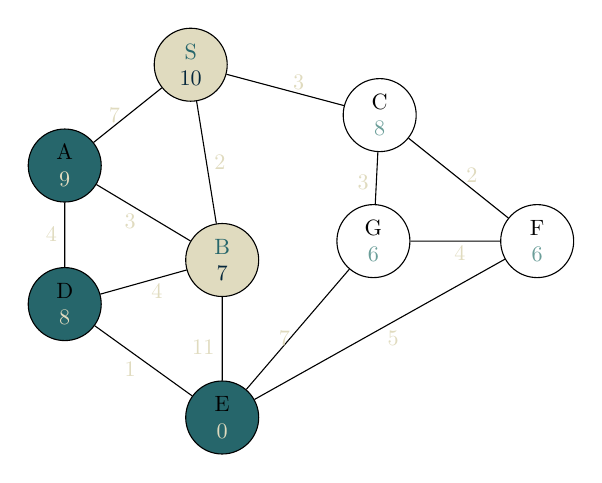
\begin{tikzpicture}[scale=0.8, every node/.style={transform shape}]
		\node [node,text width=0.5cm,fill=primary, text=darkeraccent](s){S \color{bgcolor}{10}};	
		\node [node,xshift=-2cm,yshift=-.6cm,below of=s,text width=0.5cm,fill=darkeraccent](a){A \color{primary}{9}};
		\node [node,below of=a,xshift=2.5cm,yshift=-.5cm,text width=0.5cm,fill=primary, text=darkeraccent](b){B \color{bgcolor}{7}};
		\node [node,below of=a,yshift=-1.2cm,text width=0.5cm,fill=darkeraccent](d){D \color{primary}{8}};
		\node [node,below of=s,xshift=3cm,yshift=.2cm,text width=0.5cm](c){C \color{accent}{8}};
		\node [node,below of=c,xshift=2.5cm,yshift=-1cm,text width=0.5cm](f){F \color{accent}{6}};
		\node [node,below of=c,xshift=-0.1cm,yshift=-1cm,text width=0.5cm](g){G \color{accent}{6}};
		\node [node,below of=b,yshift=-1.5cm,text width=0.5cm,fill=darkeraccent](e){E \color{primary}{0}};
		
		\draw[-](s)--node[left]{\color{primary}{7}}(a);
		\draw[-](s)--node[right]{\color{primary}{2}}(b);
		\draw[-](s)--node[right,yshift=.12cm]{\color{primary}{3}}(c);
		\draw[-](a)--node[left,yshift=-.14cm]{\color{primary}{3}}(b);
		\draw[-](a)--node[left]{\color{primary}{4}}(d);
		\draw[-](b)--node[right,yshift=-.14cm]{\color{primary}{4}}(d);
		\draw[-](b)--node[left,yshift=-.14cm]{\color{primary}{11}}(e);
		\draw[-](d)--node[left,yshift=-.14cm]{\color{primary}{1}}(e);
		\draw[-](c)--node[right,yshift=.05cm]{\color{primary}{2}}(f);
		\draw[-](c)--node[left,yshift=-.06cm]{\color{primary}{3}}(g);
		\draw[-](f)--node[right,xshift=-.14cm,yshift=-.2cm]{\color{primary}{4}}(g);
		\draw[-](f)--node[right,yshift=-.14cm]{\color{primary}{5}}(e);
		\draw[-](g)--node[left,yshift=-.14cm]{\color{primary}{7}}(e);
		\end{tikzpicture}
		
	\end{figure}
	\column{0.4\textwidth}
	\begin{figure}[h]
		Priority Queue\\*
		
		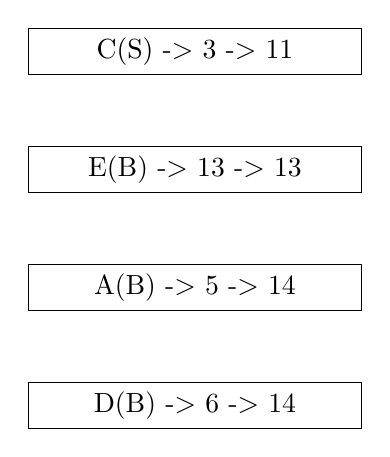
\begin{tikzpicture}
	%	\node [myBox](b1){\text{B -$>$	2 -$>$ 9}};
		\node [myBox,yshift=-.5cm](b2){\text{C(S) -$>$	3 -$>$ 11}};
		\node [myBox,below of=b2,yshift=-.5cm](b5){\text{E(B) -$>$	13 -$>$ 13}};
		\node [myBox,below of=b5,yshift=-.5cm](b3){\text{A(B) -$>$	5 -$>$ 14}};
		\node [myBox,below of=b3,yshift=-.5cm](b4){\text{D(B) -$>$	6 -$>$ 14}};

		\end{tikzpicture}
		
	\end{figure}
	
\end{columns}
\end{frame}




\begin{frame}{Example}

\begin{columns}
	\column{0.6\textwidth}
	
	\begin{figure}[h]
		
		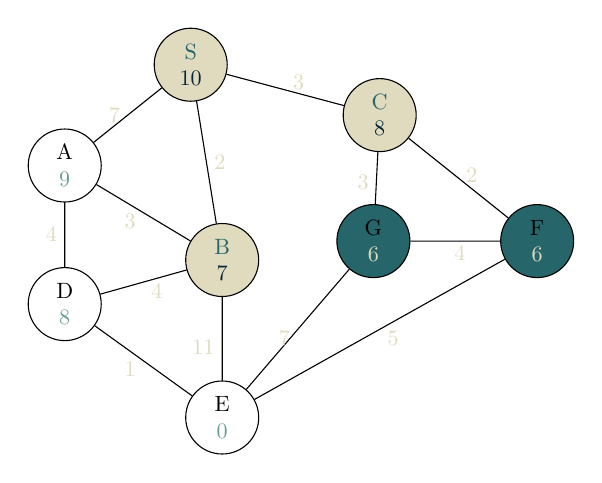
\begin{tikzpicture}[scale=0.8, every node/.style={transform shape}]
		\node [node,text width=0.5cm,fill=primary, text=darkeraccent](s){S \color{bgcolor}{10}};	
		\node [node,xshift=-2cm,yshift=-.6cm,below of=s,text width=0.5cm](a){A \color{accent}{9}};
		\node [node,below of=a,xshift=2.5cm,yshift=-.5cm,text width=0.5cm,fill=primary, text=darkeraccent](b){B \color{bgcolor}{7}};
		\node [node,below of=a,yshift=-1.2cm,text width=0.5cm](d){D \color{accent}{8}};
		\node [node,below of=s,xshift=3cm,yshift=.2cm,text width=0.5cm,fill=primary, text=darkeraccent](c){C \color{bgcolor}{8}};
		\node [node,below of=c,xshift=2.5cm,yshift=-1cm,text width=0.5cm,fill=darkeraccent](f){F \color{primary}{6}};
		\node [node,below of=c,xshift=-0.1cm,yshift=-1cm,text width=0.5cm,fill=darkeraccent](g){G \color{primary}{6}};
		\node [node,below of=b,yshift=-1.5cm,text width=0.5cm](e){E \color{accent}{0}};
		
		\draw[-](s)--node[left]{\color{primary}{7}}(a);
		\draw[-](s)--node[right]{\color{primary}{2}}(b);
		\draw[-](s)--node[right,yshift=.12cm]{\color{primary}{3}}(c);
		\draw[-](a)--node[left,yshift=-.14cm]{\color{primary}{3}}(b);
		\draw[-](a)--node[left]{\color{primary}{4}}(d);
		\draw[-](b)--node[right,yshift=-.14cm]{\color{primary}{4}}(d);
		\draw[-](b)--node[left,yshift=-.14cm]{\color{primary}{11}}(e);
		\draw[-](d)--node[left,yshift=-.14cm]{\color{primary}{1}}(e);
		\draw[-](c)--node[right,yshift=.05cm]{\color{primary}{2}}(f);
		\draw[-](c)--node[left,yshift=-.06cm]{\color{primary}{3}}(g);
		\draw[-](f)--node[right,xshift=-.14cm,yshift=-.2cm]{\color{primary}{4}}(g);
		\draw[-](f)--node[right,yshift=-.14cm]{\color{primary}{5}}(e);
		\draw[-](g)--node[left,yshift=-.14cm]{\color{primary}{7}}(e);
		\end{tikzpicture}
		
	\end{figure}
	\column{0.4\textwidth}
	\begin{figure}[h]
		Priority Queue\\*
		
		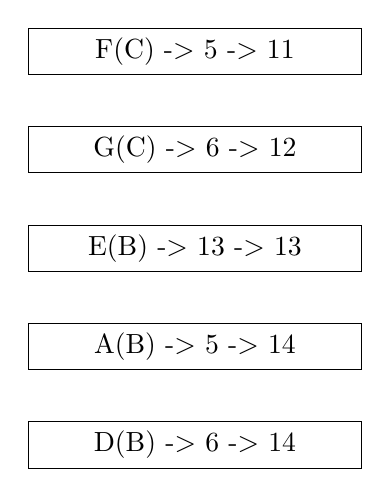
\begin{tikzpicture}
		%	\node [myBox](b1){\text{B -$>$	2 -$>$ 9}};
		\node [myBox,yshift=-.3cm](b2){\text{F(C) -$>$	5 -$>$ 11}};
		\node [myBox,below of=b2,yshift=-.25cm](b1){\text{G(C) -$>$	6 -$>$ 12}};
		\node [myBox,below of=b1,yshift=-.25cm](b5){\text{E(B) -$>$	13 -$>$ 13}};
		\node [myBox,below of=b5,yshift=-.25cm](b3){\text{A(B) -$>$	5 -$>$ 14}};
		\node [myBox,below of=b3,yshift=-.25cm](b4){\text{D(B) -$>$	6 -$>$ 14}};
		
		\end{tikzpicture}
		
	\end{figure}
	
\end{columns}
\end{frame}


\begin{frame}{Example}

\begin{columns}
	\column{0.6\textwidth}
	
	\begin{figure}[h]
		
		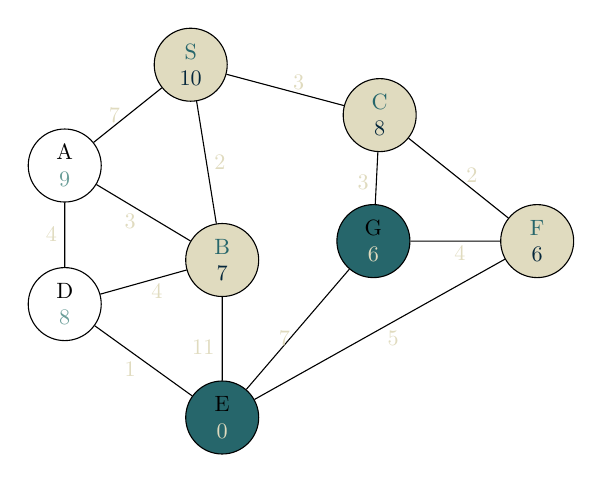
\begin{tikzpicture}[scale=0.8, every node/.style={transform shape}]
		\node [node,text width=0.5cm,fill=primary, text=darkeraccent](s){S \color{bgcolor}{10}};	
		\node [node,xshift=-2cm,yshift=-.6cm,below of=s,text width=0.5cm](a){A \color{accent}{9}};
		\node [node,below of=a,xshift=2.5cm,yshift=-.5cm,text width=0.5cm,fill=primary, text=darkeraccent](b){B \color{bgcolor}{7}};
		\node [node,below of=a,yshift=-1.2cm,text width=0.5cm](d){D \color{accent}{8}};
		\node [node,below of=s,xshift=3cm,yshift=.2cm,text width=0.5cm,fill=primary, text=darkeraccent](c){C \color{bgcolor}{8}};
		\node [node,below of=c,xshift=2.5cm,yshift=-1cm,text width=0.5cm,fill=primary, text=darkeraccent](f){F \color{bgcolor}{6}};
		\node [node,below of=c,xshift=-0.1cm,yshift=-1cm,text width=0.5cm,fill=darkeraccent](g){G \color{primary}{6}};
		\node [node,below of=b,yshift=-1.5cm,text width=0.5cm,fill=darkeraccent](e){E \color{primary}{0}};
		
		\draw[-](s)--node[left]{\color{primary}{7}}(a);
		\draw[-](s)--node[right]{\color{primary}{2}}(b);
		\draw[-](s)--node[right,yshift=.12cm]{\color{primary}{3}}(c);
		\draw[-](a)--node[left,yshift=-.14cm]{\color{primary}{3}}(b);
		\draw[-](a)--node[left]{\color{primary}{4}}(d);
		\draw[-](b)--node[right,yshift=-.14cm]{\color{primary}{4}}(d);
		\draw[-](b)--node[left,yshift=-.14cm]{\color{primary}{11}}(e);
		\draw[-](d)--node[left,yshift=-.14cm]{\color{primary}{1}}(e);
		\draw[-](c)--node[right,yshift=.05cm]{\color{primary}{2}}(f);
		\draw[-](c)--node[left,yshift=-.06cm]{\color{primary}{3}}(g);
		\draw[-](f)--node[right,xshift=-.14cm,yshift=-.2cm]{\color{primary}{4}}(g);
		\draw[-](f)--node[right,yshift=-.14cm]{\color{primary}{5}}(e);
		\draw[-](g)--node[left,yshift=-.14cm]{\color{primary}{7}}(e);
		\end{tikzpicture}
		
	\end{figure}
	\column{0.4\textwidth}
	\begin{figure}[h]
		Priority Queue\\*
		
		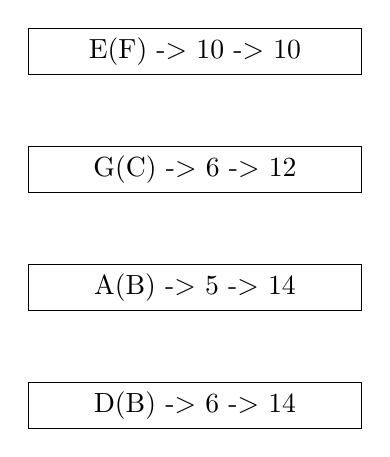
\begin{tikzpicture}
		%	\node [myBox](b1){\text{B -$>$	2 -$>$ 9}};
		\node [myBox,yshift=-.5cm](b2){\text{E(F) -$>$	10 -$>$ 10}};
		\node [myBox,below of=b2,yshift=-.5cm](b1){\text{G(C) -$>$	6 -$>$ 12}};
		%\node [myBox,below of=b1,yshift=-.5cm](b5){\text{E -$>$	10 -$>$ 13}};
		\node [myBox,below of=b1,yshift=-.5cm](b3){\text{A(B) -$>$	5 -$>$ 14}};
		\node [myBox,below of=b3,yshift=-.5cm](b4){\text{D(B) -$>$	6 -$>$ 14}};
		
		\end{tikzpicture}
		
	\end{figure}
	
\end{columns}
\end{frame}


\begin{frame}{Example}

\begin{columns}
	\column{0.6\textwidth}
	
	\begin{figure}[h]
		
		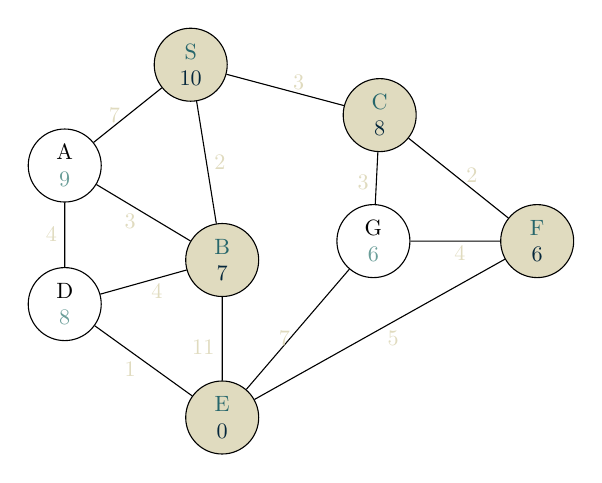
\begin{tikzpicture}[scale=0.8, every node/.style={transform shape}]
		\node [node,text width=0.5cm,fill=primary, text=darkeraccent](s){S \color{bgcolor}{10}};	
		\node [node,xshift=-2cm,yshift=-.6cm,below of=s,text width=0.5cm](a){A \color{accent}{9}};
		\node [node,below of=a,xshift=2.5cm,yshift=-.5cm,text width=0.5cm,fill=primary, text=darkeraccent](b){B \color{bgcolor}{7}};
		\node [node,below of=a,yshift=-1.2cm,text width=0.5cm](d){D \color{accent}{8}};
		\node [node,below of=s,xshift=3cm,yshift=.2cm,text width=0.5cm,fill=primary, text=darkeraccent](c){C \color{bgcolor}{8}};
		\node [node,below of=c,xshift=2.5cm,yshift=-1cm,text width=0.5cm,fill=primary, text=darkeraccent](f){F \color{bgcolor}{6}};
		\node [node,below of=c,xshift=-0.1cm,yshift=-1cm,text width=0.5cm](g){G \color{accent}{6}};
		\node [node,below of=b,yshift=-1.5cm,text width=0.5cm,fill=primary, text=darkeraccent](e){E \color{bgcolor}{0}};
		
		\draw[-](s)--node[left]{\color{primary}{7}}(a);
		\draw[-](s)--node[right]{\color{primary}{2}}(b);
		\draw[-](s)--node[right,yshift=.12cm]{\color{primary}{3}}(c);
		\draw[-](a)--node[left,yshift=-.14cm]{\color{primary}{3}}(b);
		\draw[-](a)--node[left]{\color{primary}{4}}(d);
		\draw[-](b)--node[right,yshift=-.14cm]{\color{primary}{4}}(d);
		\draw[-](b)--node[left,yshift=-.14cm]{\color{primary}{11}}(e);
		\draw[-](d)--node[left,yshift=-.14cm]{\color{primary}{1}}(e);
		\draw[-](c)--node[right,yshift=.05cm]{\color{primary}{2}}(f);
		\draw[-](c)--node[left,yshift=-.06cm]{\color{primary}{3}}(g);
		\draw[-](f)--node[right,xshift=-.14cm,yshift=-.2cm]{\color{primary}{4}}(g);
		\draw[-](f)--node[right,yshift=-.14cm]{\color{primary}{5}}(e);
		\draw[-](g)--node[left,yshift=-.14cm]{\color{primary}{7}}(e);
		\end{tikzpicture}
		
	\end{figure}
	\column{0.4\textwidth}
	\begin{figure}[h]
		Priority Queue\\*
		
		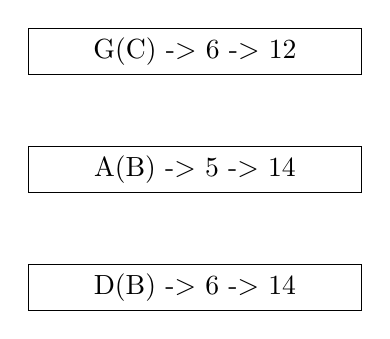
\begin{tikzpicture}
	
	
		\node [myBox,yshift=-.5cm](b1){\text{G(C) -$>$	6 -$>$ 12}};
		\node [myBox,below of=b1,yshift=-.5cm](b3){\text{A(B) -$>$	5 -$>$ 14}};
		\node [myBox,below of=b3,yshift=-.5cm](b4){\text{D(B) -$>$	6 -$>$ 14}};
		
		\end{tikzpicture}
		
	\end{figure}
	
\end{columns}
\end{frame}


\begin{frame}{Example}
	
	\begin{figure}[h]
		\centering
		\begin{tikzpicture}[scale=0.9, every node/.style={transform shape}]
		\node [node,text width=0.5cm,fill=primary, text=darkeraccent](s){S \color{bgcolor}{10}};	
		\node [node,below of=s,xshift=2.5cm,text width=0.5cm,fill=primary, text=darkeraccent](c){C \color{bgcolor}{8}};
		\node [node,below of=c,xshift=2cm,yshift=-1cm,text width=0.5cm,fill=primary, text=darkeraccent](f){F \color{bgcolor}{6}};
		\node [node,below of=b,yshift=-2cm,text width=0.5cm,fill=primary, text=darkeraccent](e){E \color{bgcolor}{0}};		
		\draw[-](s)--node[right,yshift=.12cm]{\color{primary}{3}}(c);
		\draw[-](c)--node[right,yshift=.05cm]{\color{primary}{2}}(f);
		\draw[-](f)--node[right,yshift=-.14cm]{\color{primary}{5}}(e);
		\end{tikzpicture}
		\caption{Expected shortest path}
	\end{figure}
 

\end{frame}


	
\section{Heuristic Functions}
\subsection{Exact Heuristics}
\begin{frame}
	\frametitle{Exact Heuristics}
	\begin{columns}
		\begin{column}{0.5\textwidth}
			\begin{tcolorbox}
				\large
				Using exact distance from any node $n$ to goal node as $h(n)$
			\end{tcolorbox}
		\end{column}
		\begin{column}{0.5\textwidth}
			\begin{itemize}
				\item Precompute distances between each pair of nodes
				\pause
				\item Time-consuming
				\pause
				\item Equal to Euclidean distance if there is no other node on the direct path
			\end{itemize}
		\end{column}
	\end{columns}		
\end{frame}

\subsection{Approximate Heuristics}
\subsubsection{Manhattan Distance}
\begin{frame}
	\frametitle{Manhattan Distance}
	\begin{tcolorbox}[height=0.25\textheight]
		\large
		$ h(n) =  
		\mid n.x - g.x \mid + 
		\mid n.y - g.y \mid $ 	
	\end{tcolorbox}
	\begin{itemize}
		\item Suitable for 2D grids
		\item Movement is allowed only in $x$ or $y$ axis (4 directions)
	\end{itemize}
\end{frame}

\subsubsection{Diagonal Distance}
\begin{frame}
	\frametitle{Diagonal Distance}
	\begin{tcolorbox}[height=0.25\textheight]
		\large
		$ h(n) = \max \{  
		\mid n.x - g.x \mid ,  
		\mid n.y - g.y \mid \} $ 
	\end{tcolorbox}
	\begin{itemize}
		\item Suitable for games like chess
		\item Both axial and diagonal movements are allowed (8 directions)
	\end{itemize}
\end{frame}

\subsubsection{Euclidean Distance}
\begin{frame}
	\frametitle{Euclidean Distance}
	\begin{tcolorbox}[height=0.25\textheight]
		\large
		$ h(n) = \sqrt{( n.x - g.x )^2 +
			( n.y - g.y )^2} $ 
	\end{tcolorbox}
	\begin{itemize}
		\item Suitable for graphs
		\item Movement in any direction is allowed
	\end{itemize}
\end{frame}

\section{Implementation}
\begin{frame}
	\frametitle{Implementation}
	\begin{tcolorbox}[width=\textwidth, height=0.3\textheight]
		\large
		Implementation details that can affect the performance of A*
	\end{tcolorbox}
	\begin{itemize}
		\item Breaking ties in deciding minimum element of priority queue
		\pause
		\item Alternative heap implementations of priority queue
	\end{itemize}
\end{frame}	

\subsection{Breaking Ties}
\begin{frame}
	\frametitle{Breaking Ties}
	\begin{tcolorbox}[width=\textwidth, height=0.2\textheight]
		\large
		How to break ties in priority queue?
	\end{tcolorbox}
	\begin{description}
		\item[$\bullet$ \bfseries{lowest heuristic cost}] \hfill \\ - Prefer the nodes closest to the goal
		\pause
		\item[$\bullet$ \bfseries{cross product of s-g and n-g vectors}] \hfill \\ - Prefer paths on the start-goal straight line 
		\pause
		\item[$\bullet$ \bfseries{LIFO like DFS}] \hfill \\ - Prefer new insertions to old insertions 
	\end{description}
\end{frame}

\subsection{Heap Data Structures}
\begin{frame}
	\frametitle{Which heap to use?}
	\begin{columns}[c]
		\begin{column}{0.4\textwidth}
			\begin{tcolorbox}
				\centering
				\Large
				Binary \\Heap
			\end{tcolorbox}
		\end{column}
		\begin{column}{0.1\textwidth}
			\centering VS
		\end{column}
		\begin{column}{0.4\textwidth}
			\begin{tcolorbox}
				\centering
				\Large
				Fibonacci Heap
			\end{tcolorbox}
		\end{column}
	\end{columns}
\end{frame}

\begin{frame}
	\frametitle{Which heap to use?}
	\renewcommand{\arraystretch}{2.0}
	\begin{table}[h]
		\centering
		\begin{tabular}{|p{0.27\textwidth}|p{0.2\textwidth}|p{0.18\textwidth}|p{0.2\textwidth}|}
			
			\hline
			Operation & Delete-min & Insert & Decrease-key \\
			\hline
			Binary Heap & $\Theta(\log{n})$ & $\mathcal{O}(\log{n})$ & $\mathcal{O}(\log{n})$ \\
			\hline
			Fibonacci Heap & Amortized  $\mathcal{O}(\log{n})$ & $\Theta(1)$ & Amortized $\Theta(1)$ \\
			\hline
		\end{tabular}
		\caption{Time-complexity comparisons}
	\end{table}
\end{frame}

\begin{frame}
	\frametitle{Which heap to use?}
	\begin{columns}[c]
		\begin{column}{0.4\textwidth}
			\begin{tcolorbox}[colback=darkeraccent, coltext=primary]
				\centering
				\Large
				Binary \\Heap
			\end{tcolorbox}
		\end{column}
		\begin{column}{0.1\textwidth}
			\centering VS
		\end{column}
		\begin{column}{0.4\textwidth}
			\begin{tcolorbox}[colback=accent]
				\centering
				\Large
				Fibonacci Heap
			\end{tcolorbox}
		\end{column}
	\end{columns}
\end{frame}


\section{Time Complexity}
\begin{frame}
	\frametitle{Time Complexity}
	\begin{block}{Branching Factor (b)}
		Average number of neighbours at each node
	\end{block}
	\hfill
	\pause
	\begin{block}{Depth of Solution (d)}
		Number of nodes in the shortest path
	\end{block}
	\hfill
	\pause
	\begin{tcolorbox}[width=\textwidth, height=0.2\textheight]
		\large
		Time Complexity : $\mathcal{O}(b^d)$ or $\mathcal{O}(\mid E\mid)$
	\end{tcolorbox}
\end{frame}

\section{Applications}
\begin{frame}
	\frametitle{Where do we use A*?}
	\begin{figure}
		\centering
		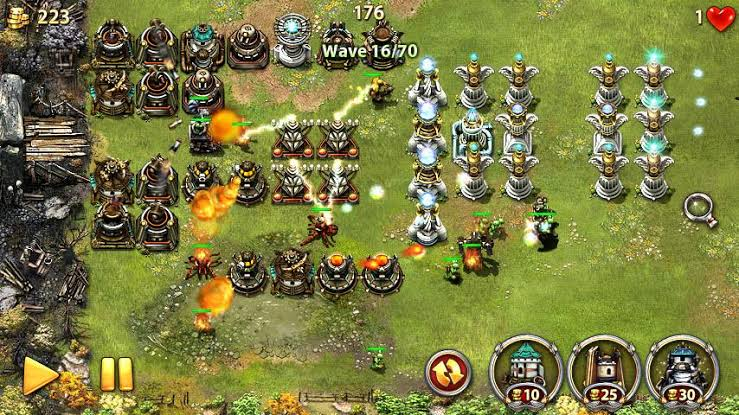
\includegraphics[width=0.7\textwidth]{towerdefense}
		\caption{Tower Defense}
	\end{figure}
\end{frame}

\begin{frame}
	\frametitle{Where do we use A*?}
	\begin{description}
		\item[$\bullet$ \bfseries{Finding shortest path in games}] \hfill \\ - mostly single source, single destination
		\pause
		\item[$\bullet$ \bfseries{Graph Traversal}] \hfill \\ - originally designed for this purpose 
		\pause
		\item[$\bullet$ \bfseries{Artificial Intelligence}] \hfill \\ - informed search algorithm for agents 
		\pause
		\item[$\bullet$ \bfseries{Navigation}] \hfill \\ - Google Maps \& other digital maps
	\end{description}
\end{frame}


\begin{frame}
	\frametitle{THE END}
	\centering
	\LARGE
	Thank You ! \\
	\Large
	Feel free to ask any questions
\end{frame}

\end{document}
